%KECReportFormat.tex
%%%%%%%%%%%%%%%%%%%%%%%%%%%%%%%%%%%%%%%%%%%%%%%%%%%%%%%%%%%%%%%%%%%%%%%%%%%
%DO NOT MAKE CHANGES IN THIS FILE

\documentclass[12pt, a4paper]{report}
\usepackage[left = 1.5in, right = 1in, top = 1in, bottom = 1in]{geometry}%for margin
\usepackage{amsfonts, amsmath, amssymb} %for mathematical equations
\usepackage{graphicx} %for images
\usepackage{times} %font Times New Roman Font
\usepackage{float} %required if you use H(strictly here) position for floats
\usepackage[skip = 8pt,tableposition=top, figureposition=bottom]{caption}%adjust spacing of captions and specify where captions are
\usepackage{hyperref} % for easy Navigation in document, also puts links in TOC, LOF, LOT...
\usepackage{setspace} %to change line spacing in some portion \singlespacing \onehalfspacing \doublespacing
\usepackage{acro} %for List of Abbrreviation and Symbol
\acsetup{first-style = short} % set to display only short form on the command \ac{}

%packages required for complex tables
\usepackage{bigstrut} 
\usepackage{multirow}

\renewcommand{\contentsname}{Table of Contents} %Change TOC Heading ... default is "Contents" 

\parindent 0pt	%removes the indent in paragraph
\setlength{\parskip}{18pt}	%for paragraph spacing
\renewcommand{\baselinestretch}{1.5}   %Line Spacing = 1.5 line-spaces

%to reduce spacing in sections
\usepackage{titlesec}
\titlespacing*{\section}{0pt}{0pt}{0pt} %left, top, bottom spacings
\titlespacing*{\subsection}{0pt}{0pt}{0pt}
\titlespacing*{\subsubsection}{0pt}{0pt}{0pt}
\titlespacing*{\paragraph}{0pt}{0pt}{0pt}
\titlespacing*{\subparagraph}{0pt}{0pt}{0pt}

%adjust fontsizes\ of sections
\titleformat*{\section}{\fontsize{14pt}{18pt}\bfseries}
\titleformat*{\subsection}{\fontsize{13pt}{18pt}\bfseries}
\titleformat*{\subsubsection}{\fontsize{12pt}{18pt}\bfseries}
\titleformat*{\paragraph}{\fontsize{12pt}{18pt}\bfseries}
\titleformat*{\subparagraph}{\fontsize{12pt}{18pt}\bfseries}

%to reduce separation between points in list
\usepackage{enumitem}
\setlist[enumerate]{nosep} % no separation between items in enumerate
\setlist[itemize]{nosep} % no separation between items in itemize
%use \vspace{-18pt} before list to reduce paragraph spacing between list and preceeding paragraph.

%Changes for Chapter Heading Spacing and formats for numbered chapters
\makeatletter
\def\@makechapterhead#1{%
  %\vspace*{50pt}%
  {  \MakeUppercase{\ifnum \c@secnumdepth >\m@ne
        \fontsize{16pt}{1}\bfseries \@chapapp \space \thechapter\vspace{5pt}\\
    \fi
    \interlinepenalty\@M
     \bfseries #1}\par\nobreak
    %\vskip 0pt
  }}
\makeatother

%%%%%%%%%%%%%%%%%%%%%%%%%%%%%%%%%%%%%%%%%%%%%%%%%%%%%%%%%%%
%to adjust Heading spacings and fonts For unnumbered chapters, TOC, LOF ...
\makeatletter
% Redefine the \chapter* header macro to remove vertical space
\def\@makeschapterhead#1{%
  %\vspace*{50\p@}% Remove the vertical space
  {\newpage \parindent \z@ \raggedright
    \normalfont
    \interlinepenalty\@M
    \center \fontsize{16pt}{1} \bfseries \MakeUppercase{#1}\par\nobreak
    %\vskip 18\p@ % adjust space after heading 18pt
  }}
\makeatother 
%%%%%%%%%%%%%%%%%%%%%%%%%%%%%%%%%%%%%%%%%%%%%%%%%%%%%%%%%%%

%%%%%%%%%%%%%%%%%%%%%%%%%%%%%%%%%%%%%%%%%%%%%%%%%%%%%%%%%%%%%%%%%%%%%%%%%%%
% newcommand for generating Cover Page
\newcommand{\KECcoverpage}
{
\begin{titlepage}
\begin{center}
\Large{\textbf{KANTIPUR ENGINEERING COLLEGE}}\\
\large{\textbf{(Affiliated to Tribhuvan University)}}\\
\large{\textbf{Dhapakhel, Lalitpur}}\\
\vfill	%vertically fill the space 
\begin{figure}[h] % h: put logo "here"
\begin{center}

\includegraphics[width=25mm, height = 25mm]{images/logo.png}
\end{center}
\end{figure}

\large{\textbf{[Subject Code: \subCode]}}\\ %Change This Line
\large{\textbf{A \MakeUppercase{\project} \MakeUppercase{\doc} ON}}\\ %Change This Line
\Large{\textbf{\MakeUppercase{\projectTitle}}}\\

\vfill	%vertically fill the space 
\large{\textbf{Submitted by:}}\\
\large{\textbf{\submittedBy}}\\
\vfill	%vertically fill the space 
\textbf{A \MakeUppercase{\project} SUBMITTED IN PARTIAL FULFILLMENT OF THE REQUIREMENT FOR THE DEGREE OF \MakeUppercase{\degree}}\\

\vfill	%vertically fill the space 
\large{\textbf{Submitted to:}}\\
\large{\textbf{\submittedTo}}\\
\vfill
\large{\textbf{\defMonth, \defYear}}
\pagebreak
\end{center}
\end{titlepage}
}
%%%%%%%%%%%%%%%%%%%%%%%%%%%%%%%%%%%%%%%%%%%%%%%%%%%%%%%%%%%%%%%%%%%%%%%
% newcommand for generating Cover Page
%Title Page
\newcommand{\KECtitlepage}
{
\begin{titlepage}
\begin{center}
\Large{\textbf{\MakeUppercase{\projectTitle}}}\\

\vfill	%vertically fill the space 

\large{\textbf{Submitted by:}}\\
\large{\textbf{\submittedBy}}\\


\ifhassupervisor % Displays Supervisor name only if \hassupervisortrue
	\vfill	%vertically fill the space 
	\large{\textbf{Supervised by:}}\\
	\large{\textbf{\supervisor}}\\
	\large{\textbf{\degSup}}\\
\fi

\vfill	%vertically fill the space 
\textbf{A \MakeUppercase{\project} SUBMITTED IN PARTIAL FULFILLMENT OF THE REQUIREMENT FOR THE DEGREE OF \MakeUppercase{\degree}}\\

\vfill	%vertically fill the space 
\large{\textbf{Submitted to:}}\\
\large{\textbf{\submittedTo}}\\
\large{\textbf{Kantipur Engineering College}}\\
\large{\textbf{Dhapakhel, Lalitpur}}\\

\vfill
\large{\textbf{\defMonth, \defYear}}
\thispagestyle{empty}\\ %to remove page number
\pagebreak
\end{center}
\end{titlepage}
}
%%%%%%%%%%%%%%%%%%%%%%%%%%%%%%%%%%%%%%%%%%%%%%%%%%%%%%%%%%%%%%%%%%%%%%
%command for copyright page
\newcommand{\KECcopyright}
{
\chapter*{Copyright}%Required only for Final Defense of Major Project
\addcontentsline{toc}{chapter}{Copyright}
The author has agreed that the library, Kantipur Engineering Collage, may make this report freely available for inspection. Moreover the author has agreed that permission for extensive copying of this report for scholarly purpose may be granted by the supervisor(s), who supervised the project work recorded herein or, in their absence, by the Head of the Department wherein this project was done. It is understood that due recognition will be given to the author of this report and to the \submittedTo, Kantipur Engineering College in any use of the material of this report. Copying or publication or other use of this report for financial gain without approval of the \submittedTo, Kantipur Engineering College and author’s written permission is prohibited.\par Request for permission to copy or to make any other use of the material in this report in whole or in part should be addressed to:

Head\\
\submittedTo\\
Kantipur Engineering College\\
Dhapakhel, Lalitpur\\
Nepal
}
%%%%%%%%%%%%%%%%%%%%%%%%%%%%%%%%%%%%%%%%%%%%%%%%%%%%%%%%%%%%%%%%%%%%%%
%command for Approval Letter
\newcommand{\KECapproval}
{
\chapter*{Kantipur Engineering College
\vskip -10pt}%Required only for Final Defense of Major Project
\begin{center}
\fontsize{12.8pt}{1} %size decreaced to adjust department name in single line
\textbf{
\MakeUppercase{\submittedTo}\\ %for department name
}
\vskip 10pt
\fontsize{16pt}{1}
\textbf{APPROVAL LETTER}
\end{center}
\vskip -16pt
\addcontentsline{toc}{chapter}{Approval Letter}%
The undersigned certify that they have read and recommended to the Institute of Engineering for acceptance, a project report entitled "\projectTitle " submitted by \\
\submittedBy \\
in partial fulfillment for the degree of \degree. \par
{\vspace{25pt}
..........................................\\
Supervisor\\
\supervisor \\
\degSup\\
\vspace{25pt}\\
..........................................\\
External Examiner\\
\external\\
\degExternal\\
\vspace{25pt}\\
..........................................\\
\hod\\
Head of Department\\
\submittedTo
\vspace{10pt}\\
Date: \defMonth\space\defDay ,\space \defYear
\singlespacing\par
} %single spacing for the texts inside {}
}

%command for list of abbreviations
\newcommand{\KECloa}
{
\chapter*{List of Abbreviations}
\addcontentsline{toc}{chapter}{List of Abbreviations}
\vskip -42pt % to reduce space due to invisivle acronym class name
{
\singlespacing
\printacronyms[include-classes=abbr, name= ]
}

}

%command for list of symbols
\newcommand{\KEClos}
{
\chapter*{List of Symbols}
\addcontentsline{toc}{chapter}{List of Symbols}
\vskip -42pt % to reduce space due to invisivle acronym class name{
{
\singlespacing
\printacronyms[include-classes=symbol, name= ]
}
}

%command to adjust toc, lof, lot spacing
\newcommand{\KECadjusttocspacings}
{
\parskip 0pt % to remove paragraph spacing in TOC, LOF ...
\renewcommand{\baselinestretch}{0.1} % to adjust line spacing in toc
\newcommand*{\noaddvspace}{\renewcommand*{\addvspace}[1]{}}
\addtocontents{lof}{\protect\noaddvspace} %remove extra vertical space in LOF
\addtocontents{lot}{\protect\noaddvspace} %remove extra vertical space in LOT
} %includes the file KecReportFormat.tex that include all necessary formattings
%%%%%%%%%%%%%%%%%%%%%%%%%%%%%%%%%%%%%%%%%%%%%%%%%%%%%%%%%%%%%%%%%%%%%%%%%%%
%Define Macros for Details of your Project
\newcommand{\project}{Major Project} %Specify "Major Project" or "Minor Project"
\newcommand{\projectTitle}{WeCare-Your Personal Health Assistance} %specify "Title" of Your Project
\newcommand{\doc}{Mid-Term Report} % specify the document you are preparing eg. "Proposal", "Mid-Term Report" or "Final Report" 
% Note that You have to sibmit "Final Report" for Pre-final defense as well.
\newcommand{\subCode}{CT755} %specify Subject of Your Project
\newcommand{\degree}{Bachelor in Computer Engineering} %specify your degree
\newcommand{\submittedBy}%Specify Names and Roll/Symbol Numbers of the Project Group Members
{
%Edit Member Names and Roll/Symbol No. and adjust width (\makebox[width]) if necessary 
\makebox[7cm]{Abhishek Gurung\hfill [91/BCT/072]}\\
\makebox[7cm]{Manjil Nepali  \hfill [105/BCT/072]}\\
\makebox[7cm]{Sagar Maharjan \hfill [118/BCT/072]}\\
\makebox[7cm]{Sovin Shrestha \hfill [126/BCT/072]}
%\makebox[9cm]{Member Name \hfill [Roll/Symbol No.]}\\
} % Note that You must write your "Symbol Numbers"(Exam Roll Numbers) for Final Defenses

\newcommand{\submittedTo}{Department of Computer and Electronics Engineering} %specify your department
\newcommand{\hod}{Er. Rabindra Khati} %specify Head ot the department
\newcommand{\defYear}{2019} %Defense Year
\newcommand{\defMonth}{July} %Defense Month- January, February, ...
\newcommand{\defDay}{15} %specify Defense Day- 1, 2, ...

\newif\ifhassupervisor
\hassupervisorfalse % to display supervisor name use command- \hassupervisortrue
 
\newcommand{\supervisor}{Supervisor's Name} % Specify Name of Supervisor for Major Project
\newcommand{\degSup}{Supervisor's Designation\\Second Line of Designation (if required)} %Specify Designation of Supervisor for Major Project, use multiple lines (\\) if necessary
\newcommand{\external}{External's Name} %Specify Name of External for Major Project (Required for Black Book)
\newcommand{\degExternal}{External's Designation\\Second Line of Designation (if required)} %Specify Name of External for Major Project (Required for Black Book) , use multiple lines (\\) if necessary


%%%%%%%%%%%%%%%%%%%%%%%%%%%%%%%%%%%%%%%%%%%%%%%%%%%%%%%%%%%%%%%%%%%%%%%%%%%

%%%%%%%%%%%%%%%%%%%%%%%%%%%%%%%%%%%%%%%%%%%%%%%%%%%%%%%%%%%%%%%%%%%%%%%%%%%
%Define Abberviations and Symbols
% NOTE that Only those Abberviations and Symbols that are included in document(using command \ac{}) will be displayed in the List of Abberviations and Symbols.

%class 'abbr': for List of Abbreviations
\DeclareAcronym{UN}{ 
  short = UN ,
  long  = United Nations ,
  class = abbr
}% declares acronym named "UN". Use \ac{UN} for short and \acl{UN} for long form. 

\DeclareAcronym{ABC}{
  short = ABC ,
  long  = Annapurna Base Camp ,
  class = abbr
}

%%%%%%%%%%%%%%%%%%%%%%%%%%%%%%%%%%%%%%%%%%%%%%%%%%%%%%%%%%%%%%%%%
% class `symbol': for List of Symbols
\DeclareAcronym{transparencyFactor}{
  short = \ensuremath{\alpha} ,
  long  = Transparency Factor ,
  sort  = Transparency Factor , % string to compare for sorting symbols... default string is the acronym name -"transparencyFactor"
  class = symbol
}% declares acronym named "transparencyFactor". Use \ac{UN} for short and \acl{UN} for long form.

\DeclareAcronym{areaOfTriangle}{
  short = \ensuremath{a} , % use \ensuremath{a} instead of $a$
  long  = Area of Triangle ,
  sort  = Area of Triangle , % string to compare for sorting symbols
  class = symbol
}
%%%%%%%%%%%%%%%%%%%%%%%%%%%%%%%%%%%%%%%%%%%%%%%%%%%%%%%%%%%%%%%%%%%%%%%%%%%%%%%%%%%%%%%%%%%%%%%%%%%%

%%%%%%%%%%%%%%%%%%%%%%%%%%%%%%%%%%%%%%%%%%%%%%%%%%%%%%%%%%%%%%%%%%%%%%%%%%
%The Document
\begin{document}

\KECcoverpage % command defined in KECReportFormat
\KECtitlepage % command defined in KECReportFormat

\pagenumbering{roman} % starts pagenumberins in Roman numerals i, ii, ...

%Copyright Page is required for FINAL REPORT only. Comment this section for other Reports.
%\KECcopyright % defined in KECReportFormat.tex	
 
  
  %Approval Page is required for FINAL(Black Book Binded) REPORT of MAJOR PROJECT only. Comment this section for other Reports. 	
 %\KECapproval % defined in KECReportFormat.tex

\chapter*{Abstract} % The summary of your report
\addcontentsline{toc}{chapter}{Abstract}%to include this chapter in TOC 
According to the World Health Organization, health is “a state of complete physical, mental and social well-being and not merely the absence of disease or infirmity.” Better health is central to human happiness and well-being. Our project "WeCare" is a prediction system that helps the user to get the information about the disease according to the symptoms they feed to the system. So that it is also called as Health Assistance application because it assists the user about the possible disease but does not give the exact information. 
\par
Traditionally, physicians or doctors use a risk calculator to assess the possibility of disease development. These calculators use fundamental information such as age, medical conditions, and more to calculate the probability of developing a certain disease.
    Main aim of our project is to develop the prediction system which predict the disease with help of data mining algorithm i.e. Feed Forward Back Propagation Neural Network 
\par
\textbf{\textit{Keywords$-$}} Health Assistance,Data Mining, Back Propagation Neural Network

\chapter*{Acknowledgment}
\addcontentsline{toc}{chapter}{Acknowledgment}%to include this chapter in TOC
This project is the outcome of inspiration and moral support of many people and for this we are grateful to them all. It’s hardly possible to list the names of all but we sincerely acknowledge their incredible contribution during the preparation. We take this opportunity to express our sincere gratitude to all those who have directly or indirectly inspired us for the completion of this project.\par
We express our gratitude towards the Computer and Electronic Department of Kantipur Engineering College for providing us the learning and working environment which was helpful to work for our team. We are very grateful to our project supervisor Shagar Upadhyay for his support in this project. Special thanks goes to Er. Bishal Thapa and Er. Shiva Gautam for providing us theoretical background, practical advice and valuable suggestions for the development of this design. We would also like to thank the library staff for providing us with the study materials needed for research purposes.
\par
%to display members name under Acknowledgement
\begin{flushright}
\vskip -20pt
\setstretch{1.2}
\submittedBy
\end{flushright}



%to adjust spacings for TOC, LOF, LOT
{
%%%%%%%%%%%%%%%%%%%%%%%%%%%%%%%%%%%%%%%%%%%%%%%%%%%%%%%%%%%%%%%%%%%%%%%%%%%
%TOC, LOF and LOT
\KECadjusttocspacings % defined in KECReportFormat.tex to adjust spacings
\makeatletter
% to add vskip of 18 point which is reduced when parskip is set to 0 in \LECadjustspacings
\def\@makeschapterhead#1{%
  %\vspace*{50\p@}% Remove the vertical space
  {\newpage \parindent \z@ \raggedright
    \normalfont
    \interlinepenalty\@M
    \center \fontsize{16pt}{1} \bfseries \MakeUppercase{#1}\par\nobreak
    \vskip 18\p@ % adjust space after heading 18pt
  }}
\makeatother 

\tableofcontents % prints table of contents
\listoffigures % prints list of figures

}
%%%%%%%%%%%%%%%%%%%%%%%%%%%%%%%%%%%%%%%%%%%%%%%%%%%%%%%%%%%%%%%%%%%%%%%%%%%



\newpage
\pagenumbering{arabic} % starts pagenumbering in arabic numerals

\chapter{Introduction}
\section{Background}\label{sec:bkgrnd}%label your section if you require to refer them somewhere else in your document.
Human health is a relative state in which one is able to function well i.e physically, mentally and live socially well-being within the environment in which one is living. The human body is an incredible machine i.e has the ability to adapt, repair itself and manage challenges throughout life. With the on-going development of world over years, human learns the symptoms of affected human and provide remedy for hazardeous diseases.\par
The health sector is of critical importance for human development, improving living standards in rural areas and for mainstreaming marginalized groups and communities. Despite significant progress in recent years, service delivery in the health sector remains weak.  Although an extensive network of primary health care centres has been constructed nationwide, it has not been functioning well in many rural areas due to lack of trained staff, drugs and medicines, etc.  The sector's overall performance has suffered due to inadequate funding for essential recurrent  expenditures, misallocation  of  resources  and  limited  capacity  for supervision and for co-ordination of the activities of other agencies providing health care services.\par


This android application entitled "WeCare-Your Personal Health Assistance" aims to be helpful application by predicting the possible diseases as Tele-medicine center. Our proposed system takes symptoms from the user as input and data mining technique is used to do provisional diagnosis as practiced in telemedicine centers. Similar to that in telemedicine center, output generated doesn't provide fully diagnosed results. The user has to consult doctor for further treatment.\par
 In  order  to  reduce the risk of disease, prediction should be done. Discovering of disease  is usually based on symptoms, physical examinations and signs of patient body. Normally, doctors are predicting disease by knowledge and experience. Discovering and predicting    diseases  is  a  difficult  task  in  medical  environment. Discovering disease from several factors is a multi-layered problem which may lead to negative presumptions and unpredictable effects. As a result, Health-care  industry  today  creates  large  amounts  of  complex  data  about  patients, hospitals resources, disease diagnosis, electronic patient records, medical devices etc. The huge amount of data is a key resource  to be processed and analyzed for knowledge extraction that enables support for cost-savings and decision making. 

\section{Problem Statement}\label{sec:ps}%label your section if you require to refer them somewhere else in your document.
Taking appointment with the doctors is very difficult in both rural an urban areas of Nepal. Like most developing nations, doctors are geographically maldistributed in Nepal. The Kathmandu valley has one doctor for 850 people but in rural areas the number is one doctor for every 150000 people. The doctor-population density in Kathmandu is estimated to be about 40 times that in rural Nepal. \par People often feel reluctant to go to hospital or physician on  minor symptoms.  However, in  many  cases, these  minor symptoms may trigger major health hazards. If they get some information about the disease they might have been suffering from, it will be helpful when they discuss their problems with the doctor later. \par People will not know the possible reasons for the disease and may be mistaken with other disease. It will be helpful to take the preventive measures if people have some idea about the disease they are suffering from. Now a day's people are busy on their daily life works so they forget to take their medicine on time, thus it could be helpful if someone notify them on time to take their medicine. So, Pill Reminder lets you create tasks with a deadline. The reminder simply reminds you when it's time to do it.   
\pagebreak
\section{Objectives}\label{sec:obj}%label your section if you require to refer them somewhere else in your document.
The major objectives are listed:
\begin{itemize}
    \item To give environment to the users to diagnose their symptoms. 
    \item To list out provisional diagnosed diseases.
    \item To help users take an active role in meaning their health by providing objective healthcare information.
\end{itemize}
\section{Applications}\label{sec:app}%label your section if you require to refer them somewhere else in your document.
This developed application enables users to make sense of symptoms and recognition of disease by decision algorithm. This project has wide use in various fields.\par
As in rural areas, it might have happened so many times that people may need doctors help immediately, but they are not available due to some reason. This project allows user to get instant guidance on their health related problems. This app is a tool for user to check their symptoms, find trusted information and probable diseases with questionnaire based on the symptoms. This project is not limited to diseases prediction only, it suggests basic preventive measures and overview of the disease. Users can take immediate action. This project has wide area of application use in telemedicine centers. It can be easily access by nursing home staffs, sometimes parents and patient themselves. Users can get quick instant guidance of disease with preventive measures.\par
This project also provides the functionality of pill reminder, where users can get instant  notifications of time and medicine to be taken according to their prescriptive noted schedule. As taking of medicine pill in time, during of sickness has great affect in health, pill reminder can be very useful to users.

\pagebreak
\section{Features}\label{sec:feat}%label your section if you require to refer them somewhere else in your document.
The features are listed: 
\begin{itemize}
    \item Provides suggestions and informs about the possible occurence of disease based on the symptoms ans users information.
    \item User friendly interface.
    \item Suggest basic preventive measures and overview of disease.
    \item Works as pill reminder.
\end{itemize}
\section{Feasibility Analysis}\label{sec:fa}%label your section if you require to refer them somewhere else in your document.
\subsection{Economic Feasibility}
Economic Feasibility is the cost and logistical outlook for a business project and is carried out to check the economic impact to the organization by the use of this system. The amount of fund that the company can invest for system is limited.

\subsection{Technical Feasibility}
This study is carried out to check technical requirements of the system. Any system developed must not have a high demand on the available technical resources as this may lead to high demands being placed on the client. This project doesn't incorporate the use of complex hardware. The technology required for the project is practical and necessary technical resources and expertise are assured.

\subsection{Operational Feasibility}
Operational feasibility is the ability to utilize, support and perform the necessary tasks of a system or program. The aspect of study is to check the level of acceptance of the system by the user. This system has been developed with users in mind. With the use of android technology, the system is easy to use and operate. The effective operation of the system can be achieved in required health purpose application. Greater level of user-friendliness and high performance of the proposed system can be achieved.

\section{System Requirements}\label{sec:sr}%label your section if you require to refer them somewhere else in your document.
\subsection{Software Requirements}
\begin{itemize}
    \item Android Studio
    \item Java
    \item Python
    \item Flask
\end{itemize}

\subsection{Hardware Requirements}
\begin{itemize}
    \item Android Mobile
\end{itemize}


\chapter{Literature Review}
There are different areas in medicine where an expert system has  been  designed  and  implemented. Numerous works has been done related to disease diagnosis using different data mining techniques. 


\section{Previous Work On Medical Expert System}
\subsection{MYCIN}
MYCIN is the name of a decision support system developed by Stanford University in the early-to mid-seventies, built to assist physicians in the diagnosis of infectious diseases. The system (also known as an "expert system") would ask a series of questions designed to emulate the thinking of an expert in the field of infectious disease (hence the "expert-"), and from the responses to these questions give a list of possible diagnoses, with probability, as well as recommend treatment (hence the "decision support-").\par 
MYCIN is an AI program designed:
\begin{itemize}
    \item to provide expert level solutions to complex problems
    \item to be understandable
    \item to be flexible enough to accommodate new knowledge easily
\end{itemize}
MYCIN was designed to provide advice through a consultative dialogue, which sometimes refer to it as a consultation system.

\begin{figure}[H]
\begin{center}
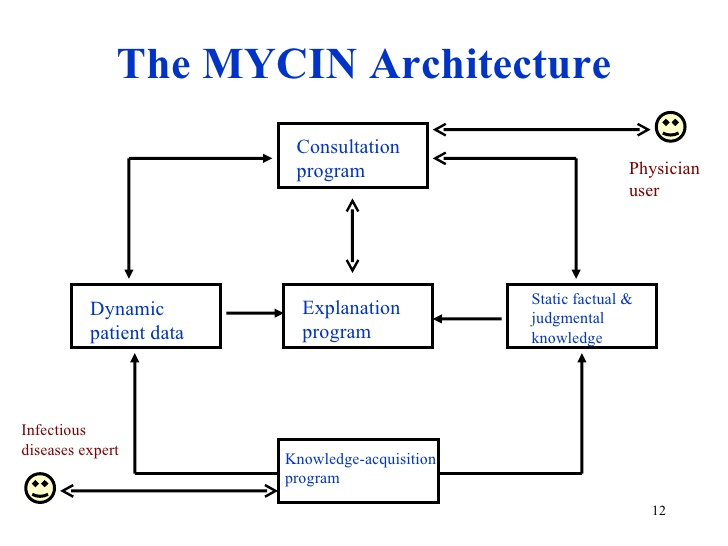
\includegraphics[width=90mm, height = 80mm]{images/mycin.jpg}
\caption{MYCIN Architecture(Source: slideshare.net)}
\end{center}
\end{figure}
\subsection{Chronic Kidney Disease Prediction Using Back Propagation Neural Network Algorithm}
This system of neural network accepts disease-symptoms as input and it is trained according to various training algorithms. Levenberg, Bayesian regularization, Scaled Conjugate and Resilient back propagation algorithm are discussed here. After neural network is trained using back propagation algorithms, this trained neural network system is used for detection of kidney disease in the human body. The back propagation algorithms presented here have capacity for distinguishing amongst infected patients or non-infected person.
\section{Automated Disease Prediction System (ADPS): A User Input-based Reliable Architecture for Disease Prediction}
Automated  Disease  Prediction System  (ADPS)  that  relies  on guided  (to be  described later)  user input.  The system  takes input from the user and provides a list (topmost diseases have greater  likelihood  of occurrence)  of  probable  diseases.  The accuracy of ADPS has been evaluated extensively. It ensured an average of 14.35\% higher accuracy in comparison with the existing solution. \par
In  this  paper,  the  contribution  includes  proposing  a  new disease prediction framework (ADPS) that takes into account symptom  names  as  well  as  other  vital  parameters to improve disease prediction accuracy and  proposing  techniques  to allow  greater  linguistic  diversity  so  that  users  do  not  feel uncomfortable while giving input. \par
It is presumed that the user will give text input in one sentence describing  a  single  symptom  at  a  time  (guideline  for  user input). Subsequent symptoms can be added in new lines. After getting user input, the system will scan through each line and tag  each  word  according  to  their relevant  parameter.  Then after performing certain computations (to be described later) the  system  will  return  a  list  of  possible  diseases  ordered according to the likelihood of their occurrences.

\section{Neural Network Based Intelligent System for Predicting Heart Disease}

This paper proposed an intelligent automated system incorporating  the  techniques of data mining with machine learning in order to make decisions. Medical practitioners are being assisted by  the  automated  systems  for  providing effective  treatment  [18].  Data  mining  techniques  involves  a combination  of  statistical  methods  with  machine  learning algorithms  .Data  mining  techniques  help  the  system  in analyzing the symptoms and machine learning methodshelp in  predicting  the  disease  based  on  the  analysis  performed [13,20].  The  advantage  of  this  automated  system  is  that  it predicts the  disease  in  a  less  amount  of  time as  well  in less cost.  Therefore,  more  research  is  carried  out  in  the  field  of machine   intelligence   to   improvise   the   system   for   an effective   prediction.   This   paper   proposed   an   intelligent system    developed    using    the    concept    of    Multilayer Perceptron Neural Network with Back Propagation Algorithm,  as a practitioner  needs  to  make  a  decision  from multiple inputs such as current and previous medical history of  a  patient.  \par Neural  networks  are  proved  to  be  effective  in making decisions by predicting the data. As the inputs used in  predicting  the  disease  are  more  in  number  and  diagnosis has to be performed at different stages, Multilayer Perceptron  based  neural networks  are  used  in this  proposed system.  Neural  Network  extends  its  predictive  capability  at different  hierarchical  levels  in  a  multi-layered  structure  of networks.  This  multi-layered  structure helps  in  selecting features from the dataset at different scales in order to refine them  into  more  specific  features.  To  facilitate  this,  the concept of Multi-layer Perceptron Neural Network has been introduced through the implementation of Back-propagation algorithm  for  efficient  diagnosis  of  heart  disease.  In  this paper, 14 attributes are used as inputs for training the system of  neural  networks  for  diagnosing  heart  disease  risk  level using multi-layered network.Traditional   diagnosing   approaches   have   no proper automated   tools   use   for   the   purpose   of   heart   disease diagnostic   system.   The   commonly   used   data   mining algorithms for predicting diseases are: Genetic algorithm, K-means algorithm, MAFIA algorithm. Several methods proposed the implementation of classification  algorithms  in  diagnosis  of  heart  disease  and resulted with an accuracy of 88.33%





 
\chapter{Equations}

\section{Basics of Equations}
Mathematical expression within text can be written as $ y=mx+c $. In separate line as $$ ax + by + c = 0 $$
Some latex mathmatics examples:\\
Superscript:\\
$x^3$
$$x^3$$
$$x^{3x+4}$$
$$x^{{{3x+4}^4}+5}$$
Subscript:
$$x_{13}$$
${x_1}_2$
$${{{x_1}_2}_3}$$
Greek letters
$$\pi$$
$$\alpha$$
$\alpha A$
$\beta$
$\beta B$
$\delta$
$\gamma$
$\vartheta$
$\Theta$
$\phi$
$\varphi$
$\Phi$ 
trigonometric:
$y=\sin(\pi)$
Log:
$y=\log(\pi)$
$y=\ln(\pi)$
$y=\log_{10}$
Square root:
$\sqrt{2}$
$\sqrt[3]{4}$
$\sqrt{x^2+y^2}$
$\sqrt[3]{x^2+y^2}$
$\sqrt{\sqrt[3]{x^2+y^2}}$
Fraction:
About 2/3 of the class is full.
About $\frac{2}{3}$ of the class is full.
About $\displaystyle{\frac{2}{3}}$ of the class is full.
About $\displaystyle{\frac{\sqrt{\sqrt[3]{x^2+y^2}}}{\sqrt{x^2+x+1}}}$ of 
About $\displaystyle{\frac{2}{1+\sqrt{\sqrt[3]{x^2+y^2}}}}$ of the class is full.

Reserved characters:
$\{a,b,c\}$
\$20
$10\% of 100 is 100$
$10\,\,\,\% \;\;\; of \,\,\,100 \quad\qquad is\:\:\: 100$


Braket Style:
$3(\frac{2}{3})$
$3\left(Hello(\frac{2}{3})\right)$
$3\left\{Hello(\frac{2}{3})\right\}$
$3\left\{Hello(\frac{2}{3})\right.$
$3\left.Hello(\frac{2}{3})\right.$
$\left.\frac{dy}{dx}\right|_{x=1}$
( \big (  \Big (  \Bigg( 
$3(\frac{2}{3})$
$3\Big(\frac{2}{3}\Big)$

Equation:
\begin{equation} % for equations with equation numbers
% no need use $ sign
E=mc^2 
\end{equation}

\begin{equation*}
% no need use $ sign
E=mc^2 
\end{equation*}

\[
E=mc^2
\]

\begin{eqnarray}
E=mc^2 \label{eqn:mc2} \\ %labels are useful for referencing
E=mc^4\\
E=mc^7 
\end{eqnarray}

\begin{eqnarray*}
E=mc^2 \\
E=mc^4\\
E \approx \pm (mc^7 +3)\\
E \approx \pm (mc^7 +3)
\end{eqnarray*}
\begin{eqnarray}
E &=& mc^2 \\
E &=& mc^4 \nonumber \\
E &\approx& \pm (mc^7 +3)
\end{eqnarray}
Limit:
$\lim \limits_{x \to a} f(x)$\\
$\lim \limits_{x \to a} \frac{f(x)-f(a)}{x-a}=f'(a)$
Integration:
$\int$\\
$\int(\quad sin\quad x\quad dx= ) $\\
$\displaystyle{\int(\quad sin\quad x\quad dx= )} $
$\displaystyle{\int^b_a(\quad sin\quad x\quad dx= )} $
$\displaystyle{\int^b_a\: x^2\: dx\:=\left[\frac{x^3}{3}\right]^b_a} $
%$\displaystyle{\iiint^b_a\: x^2\: dx\: dy \: dz \:=\lim \limits_{x \to a}\left[\frac{x^3}{3}\right]^b_a} $


Summation:
$\displaystyle{\sum_{n=1}^{10}}$
$\displaystyle{\int^b_a\: f(x)\: dx\:=\lim \limits_{x \to \infty}\displaystyle{\sum_{K=1}^{10}f(x_k).\delta x}} $

\section{Referencing the Equation}
The Equation can be referenced using labels. example Equation \ref{eqn:mc2} of page \pageref{eqn:mc2} is referenced here.
LaTeX is the de facto standard for the communication and publication of scientific documents. LaTeX is available as free software.

\chapter{Listing Examples}
Here are some examples of listing\\
\textbf{Ordered List Technique:}\\
Listing Technique 1:
\vspace{-18pt} %use \vspace{-18pt} before list to reduce paragraph spacing between list and preceeding paragraph. 
\begin{enumerate}
\item Pencil
\item Paper
\item Calculator
\item Notebook
	\begin{enumerate}
	\item Assignment
		\begin{enumerate}
		\item Test
			\begin{enumerate}
			\item Test 1
			\item Test 2
			\end{enumerate}
		\item Quiz
		\end{enumerate}
	\item Classwork
	\end{enumerate}
\end{enumerate}

Listing Technique 2:
\vspace{-18pt}
\begin{itemize}
\item Pencil
\item Paper
\item Calculator
\item Notebook
	\begin{itemize}
		\item Assignment
		\begin{enumerate}
		\item Test
			\begin{itemize}
			\item Test 1
			\item Test 2
			\end{itemize}
		\item Quiz
		\end{enumerate}
	\item Classwork
	\end{itemize}
\end{itemize}

Listing Technique 3:
\vspace{-18pt}
\renewcommand{\labelenumii}{\Alph{enumii}}
\renewcommand{\labelenumiii}{\Roman{enumiii}}
\renewcommand{\labelenumiv}{\roman{enumiv}}
\begin{enumerate}
\item Pencil
\item Paper
\item Calculator
\item Notebook
	\begin{enumerate}
	\item Assignment
		\begin{enumerate}
		\item Test
			\begin{enumerate}
			\item Test 1
			\item Test 2
			\end{enumerate}
		\item Quiz
		\end{enumerate}
	\item Classwork
	\end{enumerate}
\end{enumerate}

\section{The Subsections}

LaTeX  is a document preparation system for the communication and publication of scientific documents. \par It is most often used for medium-to-large technical or scientific documents but it can be used for almost any form of publishing.
as said in \ref{sec:bkgrnd} of page no. \pageref{sec:bkgrnd}
LaTeX is the de facto standard for the communication and publication of scientific documents. LaTeX is available as free software.

\subsubsection{The subsubsection}
LaTeX  is a document preparation system for the communication and publication of scientific documents. \par It is most often used for medium-to-large technical or scientific documents but it can be used for almost any form of publishing.

LaTeX is the de facto standard for the communication and publication of scientific documents. LaTeX is available as free software.

\paragraph{The paragraph}
\ LaTeX  is a document preparation system for the communication and publication of scientific documents. \par It is most often used for medium-to-large technical or scientific documents but it can be used for almost any form of publishing.
\subparagraph{The subparagraph}
\ LaTeX  is a document preparation system for the communication and publication of scientific documents. \par It is most often used for medium-to-large technical or scientific documents but it can be used for almost any form of publishing.

\chapter{Example abbr and symbols}
\section{Abbr}
 Here is an example of writing abbreviations 
 \ac{ABC} is abbr of \acl{ABC}
 \ac{UN} is abbr of \acl{UN} 
\section{Symbols}
Now the symbol \ac{transparencyFactor} is the \acl{transparencyFactor}
 \ac{areaOfTriangle} is abbr of \acl{areaOfTriangle}
 Note that only those abbrs and bymbols that are included in the text will be listed in List of Abbr/Symbols.
 
\chapter{Citation Example}
\section{Citation and compiling bib file}
This is an example of citing texts \cite{Li2014}. This is second citation \cite{Yasir2014} The first cited reference will be numbered "1", second "2" and so on. Only those cited in the document will be listed in the reference section.

Note that to compile documents with reference correctly, you need to follow following steps:
\vspace{-18pt}
\begin{enumerate}
	\item Run pdfLatex (or Quick build)
	\item Run Bibtex 
	\item Run pdflatex 2 times
\end{enumerate}
 
Tation eirmod iracundia sea no, duo no aliquando elaboraret. Qui ut legere mucius, dolore efficiendi definitionem quo ex. Usu te falli similique posidonium, eum eu dicat aeterno phaedrum, te paulo deleniti ius. Pro te aliquam platonem, eos ea dolore phaedrum. Graece honestatis sit at, nec id ubique legendos.
Detracto suavitate id per, no est putent accusata quaestio, purto quaeque oporteat ei sea. Id eam erat affert, ex has summo inimicus partiendo. Option aliquam imperdiet ius ex. Efficiendi omittantur in mea, id usu tacimates rationibus. Ei accusamus dissentias vix, eos aperiam percipit id.

Mea cu vitae noluisse. Tation eirmod iracundia sea no, duo no aliquando elaboraret. Qui ut legere mucius, dolore efficiendi definitionem quo ex. Usu te falli similique posidonium, eum eu dicat aeterno phaedrum, te paulo deleniti ius. Pro te aliquam platonem, eos ea dolore phaedrum. Graece honestatis sit at, nec id ubique legendos.
Detracto suavitate id per, no est putent accusata quaestio, purto quaeque oporteat ei sea. Id eam erat affert, ex has summo inimicus partiendo. Option aliquam imperdiet ius ex. Efficiendi omittantur in mea, id usu tacimates rationibus. Ei accusamus dissentias vix, eos aperiam percipit id.

%Reference
\renewcommand\bibname{References} % Change heading to References
\bibliographystyle{IEEEtran} % to use IEEE Format for referencing
\addcontentsline{toc}{chapter}{References} % to add references in TOC
\bibliography{library} % specify the .bib file containing reference information 

%Comment this Chapter if you do not need to include Appendix.
\chapter*{Appendix}
\addcontentsline{toc}{chapter}{Appendix}
Appendix Text Comes Here

\end{document}
